\documentclass{standalone}
\usepackage{tikz}
\usepackage{ctex,siunitx}
\setCJKmainfont{Noto Serif CJK SC}
\usepackage{tkz-euclide}
\usepackage{amsmath,mhchem}
\usetikzlibrary{patterns, calc}
\usetikzlibrary {decorations.pathmorphing, decorations.pathreplacing, decorations.shapes,}
\begin{document}
\small
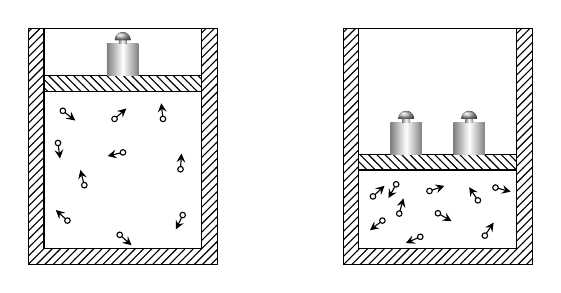
\begin{tikzpicture}[>=stealth,scale=1.0]
  % \useasboundingbox(-1,-2)rectangle(8,6);
  \begin{scope}
  \draw[pattern=north east lines](-1.2,0)--(1.2,0)--(1.2,3)--(1,3)--(1,0.2)--(-1,0.2)--(-1,3)--(-1.2,3)--cycle;
  \draw(-1.2,3)--(1.2,3);
  \draw[pattern=north west lines](-1,2.2)rectangle(1,2.4);
  \fill[left color=gray,right color=gray,middle color=white](-0.2,2.4)rectangle(0.2,2.8);
  \fill[left color=gray,right color=gray,middle color=white](-0.05,2.85)rectangle(0.05,2.8);
  \fill[ball color=lightgray](-0.1,2.85)arc(180:0:0.1)--cycle;
  \foreach \x/\y in {
    -0.760/1.951,
    -0.822/1.543,
    -0.488/1.007,
    -0.702/0.557,
    -0.038/0.376,
    0.762/0.627,
    0.734/1.209,
    0.511/1.848,
    -0.104/1.848,
    0.003/1.423%
  }
  {
    \draw[->](\x,\y)--++(360*rnd:0.2);
    \draw[fill=white] (\x,\y) circle (1pt);
  }
  \end{scope}
  \begin{scope}[xshift=4cm]
  \draw[pattern=north east lines](-1.2,0)--(1.2,0)--(1.2,3)--(1,3)--(1,0.2)--(-1,0.2)--(-1,3)--(-1.2,3)--cycle;
  \draw(-1.2,3)--(1.2,3);
  \draw[pattern=north west lines](-1,1.2)rectangle(1,1.4);
  \fill[left color=gray,right color=gray,middle color=white](0.6,1.4)rectangle(0.2,1.8);
  \fill[left color=gray,right color=gray,middle color=white](0.35,1.85)rectangle(0.45,1.8);
  \fill[ball color=lightgray](0.3,1.85)arc(180:0:0.1)--cycle;
  \fill[left color=gray,right color=gray,middle color=white](-0.6,1.4)rectangle(-0.2,1.8);
  \fill[left color=gray,right color=gray,middle color=white](-0.45,1.85)rectangle(-0.35,1.8);
  \fill[ball color=lightgray](-0.5,1.85)arc(180:0:0.1)--cycle;
  \foreach \x/\y in {
    -0.527/1.018,
    -0.822/0.864,
    -0.488/0.646,
    -0.702/0.557,
    -0.221/0.351,
    0.599/0.366,
    0.734/0.976,
    0.511/0.814,
    -0.104/0.933,
    0.003/0.650%
  }
  {
    \draw[->](\x,\y)--++(360*rnd:0.2);
    \draw[fill=white] (\x,\y) circle (1pt);
  }
  \end{scope}
  
\end{tikzpicture}
\end{document}